\cleardoublepage

\section{项目实施方案}

\subsection{软件需求分析}

本项目的目标是实现一个高效的工业场景渲染系统,
以下是针对关键需求的分析:

\par (1)\textbf{工业模型导入及数据预处理要求:}  
系统需要支持包含数亿级多边形的工业模型导入,
并确保数据预处理与加载过程在 1 小时内完成。
同时,内存占用不得超过 24GB。
为此,系统应具备高效的流式加载机制以及对大规模模型的分布式存储
和处理能力,以确保能够在有限时间内完成复杂数据的处理和加载。

\par (2)\textbf{运行时性能要求:}  
在运行时,系统显存占用不超过 8GB,
且渲染帧率需稳定在 30 FPS 左右。
此外,系统应保持较高的画面质量,
确保渲染结果与原始模型的视觉差异控制在可接受范围内。
这要求系统具备先进的 LOD(细节层次)管理与流式加载策略,
通过合理的显存管理与优化技术,保证高效渲染同时不超过显存限制。

\par (3)\textbf{与现有技术对比:}  
在帧率、显存占用、内存占用、预处理时间以及画面保真度
等关键性能指标上,本项目应至少达到与虚幻引擎 Nanite 相当的水平,
并在部分方面实现超越。例如,优化流式加载与 LOD 策略,
使得系统能够在相同硬件上实现更高效的运行,
同时降低预处理时间和显存占用。

\par (4)\textbf{鲁棒性与适应性要求:}  
系统需要具有较强的鲁棒性,能够适应不同类型的工业场景及 CAD 模型,
并能根据不同硬件配置进行优化。
为此,系统应具备灵活的硬件适配能力,
并支持动态调整渲染管线与内存使用策略,
确保在不同硬件环境下都能达到预期性能。

\subsection{项目整体架构}

\par 本项目整体可划分为预处理阶段与运行时阶段,  
如\autoref{fig:流程}所示。预处理阶段负责将原始模型从磁盘加载至内存,  
并完成模型划分与简化。包括将模型划分为多个簇(Meshlet),  
为每个子模型生成多级 LOD,并将处理结果组织成适合流式加载的结构,  
存储于 CPU 内存中,为运行时动态加载做准备。

\par 在运行时阶段,本项目主要负责几何模块与流式加载模块。  
其中,几何模块用于生成 G-Buffer,为后续光照计算等阶段提供基础数据。  
在任务着色器(Task Shader)中,还将评估当前视角所需的几何数据,  
以指导流式加载阶段的资源调度。  
流式加载模块则根据几何模块的需求,将对应的场景页按需加载至 GPU 内存,  
实现高效的数据管理与渲染支持。  
渲染管线中其余模块(如绘制指令预处理、光照与后处理等)  
由原自研引擎提供支持。

\begin{figure}[ht]
    \centering
    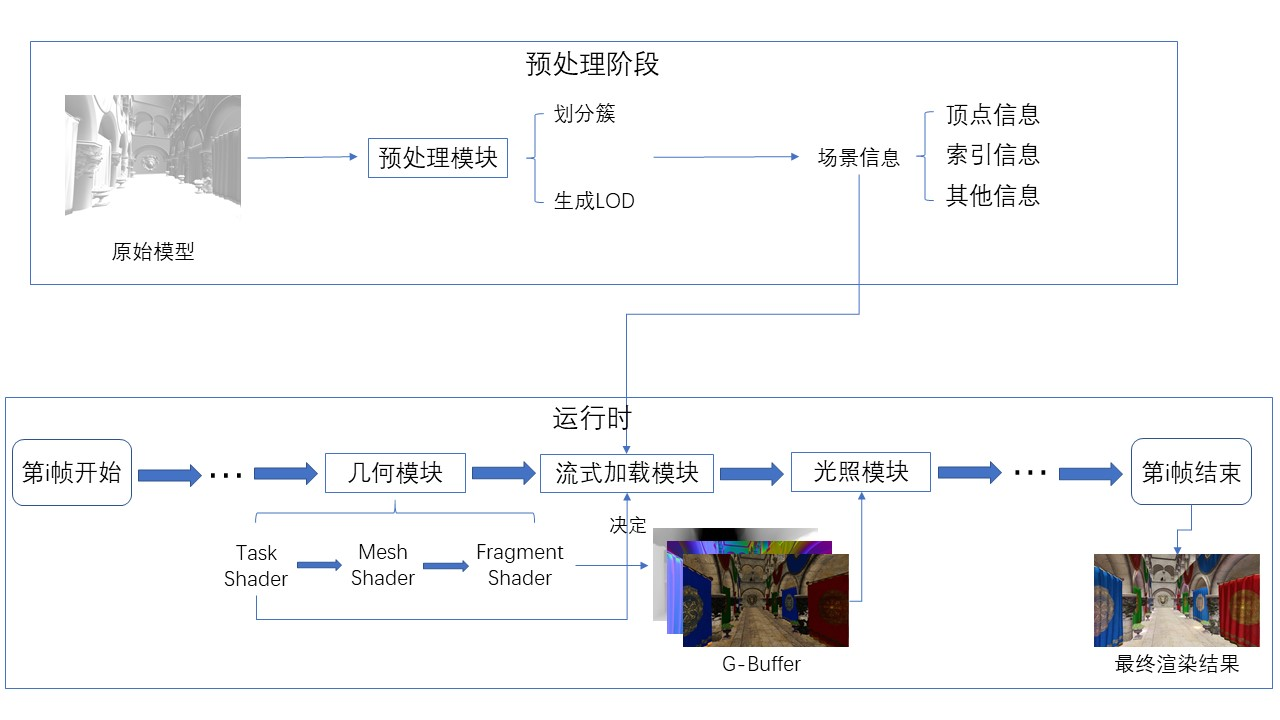
\includegraphics[width=\linewidth]{流程.jpg}
    \caption{\label{fig:流程}项目流程图}
\end{figure}

\par 综上所述,本项目在原有引擎渲染管线基础上,  
主要负责对几何模块进行修改,新增流式加载模块,并在预处理阶段  
实现了模型划分簇与生成 LOD 的功能。
通过这些改进,原渲染管线的性能得到了显著优化,  
帧率明显提升,显存占用有所降低,同时保持了良好的画面保真度。

\section{基于簇的 GPU 驱动渲染管线}

\subsection{引言}

GPU 驱动的渲染管线是一种通过 GPU 完成大部分渲染任务的渲染架构,
与传统的 CPU 驱动渲染管线相比,
GPU 驱动渲染管线能够显著提高渲染效率,
尤其在处理复杂或大规模场景时。
其核心思想是将大量渲染计算和数据处理任务交给 GPU 执行,
充分利用 GPU 强大的并行计算能力,从而加速渲染过程。

在传统的 CPU 驱动渲染管线中,
CPU 通常承担着场景遍历、物体剔除、LOD 管理等任务,
而 GPU 主要负责图形的绘制和光照计算等工作。
然而,随着图形渲染需求的提升,
CPU 驱动渲染管线的性能瓶颈逐渐显现,
特别是在处理大规模场景时,
CPU 的计算负担较重,出现渲染性能下降等问题。

而在 GPU 驱动的渲染管线中,
许多原本由 CPU 执行的任务(如剔除计算、LOD 选择等)
都转移到 GPU 上,这样可以减少 CPU 的负担,
使得 GPU 能够在更高效的并行计算模式下进行工作。

本项目除了流式加载模块中涉及到 CPU 与 GPU 之间的通信外,
其余操作均在 GPU 上实现。
与此同时,本项目引入了任务着色器(Task Shader)
和网格着色器(Mesh Shader)组成的新型渲染管线,
代替了传统的计算着色器(Compute Shader)、顶点着色器
(Vertex Shader)和几何着色器(Geometry Shader)的组合。
通过将渲染单元组织为簇(Meshlet)并以簇为单位进行处理,
进一步提升了渲染性能和灵活性。

\subsection{基于簇的渲染}

基于簇的渲染最早由育碧(Ubisoft)在游戏《刺客信条:大革命》
(Assassin's Creed Unity)中提出。
该方法将最小的剔除单元从传统的实例
(instance)替换为簇,每个簇包含64个三角形,
一个实例可以包含多个簇。
通过这种细粒度的剔除方式,
渲染引擎能够根据簇的可见性进行精确剔除,避免了
传统基于实例的剔除方法中对大范围不必要的几何数据进行处理。
对于复杂模型,
这种做法能减少需要绘制的几何体数量,
从而显著降低渲染管线中的计算负担。

本项目在预处理模块中实现了簇的划分,并设计了基于簇的渲染管线, 
有效提升了渲染性能。

\subsubsection{簇的划分} \label{subsubsec:cluster division}

簇的划分是本项目预处理阶段的关键步骤之一,
为了提高渲染效率,
本项目使用了第三方库 MeshOptimizer 来实现这一过程。(引用 MeshOptimizer 库)
MeshOptimizer 是一个高效的网格优化库,
提供了各种优化算法,可以有效地对网格进行简化和组织,
从而提高 GPU 渲染的性能。
在具体实现中,本项目规定每个簇最多由 64 个顶点 和 124 个三角形 组成。
这样的划分方式有助于平衡簇的大小和渲染效率。(引用为什么采用64个顶点)

\subsubsection{基于簇的剔除} \label{subsubsec:cluster culling}

基于簇的剔除是在任务着色器中进行的,剔除可分为视锥剔除和圆锥剔除。

其中,视锥剔除是指通过测试模型的包围球与视锥体的关系,
判断模型是否位于当前视锥内。
每一个簇都拥有自己的包围球(Bounding Sphere),
可以通过测试包围球与每个视锥平面的关系,
来判断该簇是否可能在相机的视锥范围内。
如果包围球完全在视锥体外,则该簇可以被剔除,避免不必要的渲染计算。

而圆锥剔除则是通过将簇的可见性表达为一个圆锥形状来进行判断,
圆锥的范围包含了簇的所有法线方向。
具体而言,如果相机的视角方向与圆锥范围内的所有法线方向的点积均为负数,
则说明该簇背对着相机,因此可以整体剔除,不需要渲染。
为了便于进行圆锥剔除,MeshOptimizer 库在预处理阶段会为每个簇生成
相应的圆锥信息,包括圆锥的顶点、轴和定角等参数,
这些信息可以直接用于运行时的剔除操作,大大提高了渲染效率。

\subsubsection{基于簇的网格着色器渲染管线}

网格着色器是基于簇的渲染工作流程中的关键步骤之一。
在这一阶段,任务着色器剔除后的簇将被并行处理,
网格着色器负责对簇进行顶点变换、图元组装等操作。
每个簇包含多个顶点和图元,网格着色器能够高效地并行处理多个簇,
显著减少传统渲染管线中的处理开销。

经过网格着色器处理后,簇将传递给片段着色器,
这是工作流程的最后一步。
片段着色器根据顶点的颜色、法线、纹理坐标等信息,
计算每个像素的位置、法线和颜色等,用于后续的光照计算。
网格着色器与片段着色器的协作,
使渲染管线在处理大规模网格时保持高效且灵活。

\subsection{测试分析报告}

本项目实现了簇的可视化功能,并在多个场景中进行了测试,
如\autoref{fig:Meshlet}所示。

\begin{figure}[ht]
    \centering
    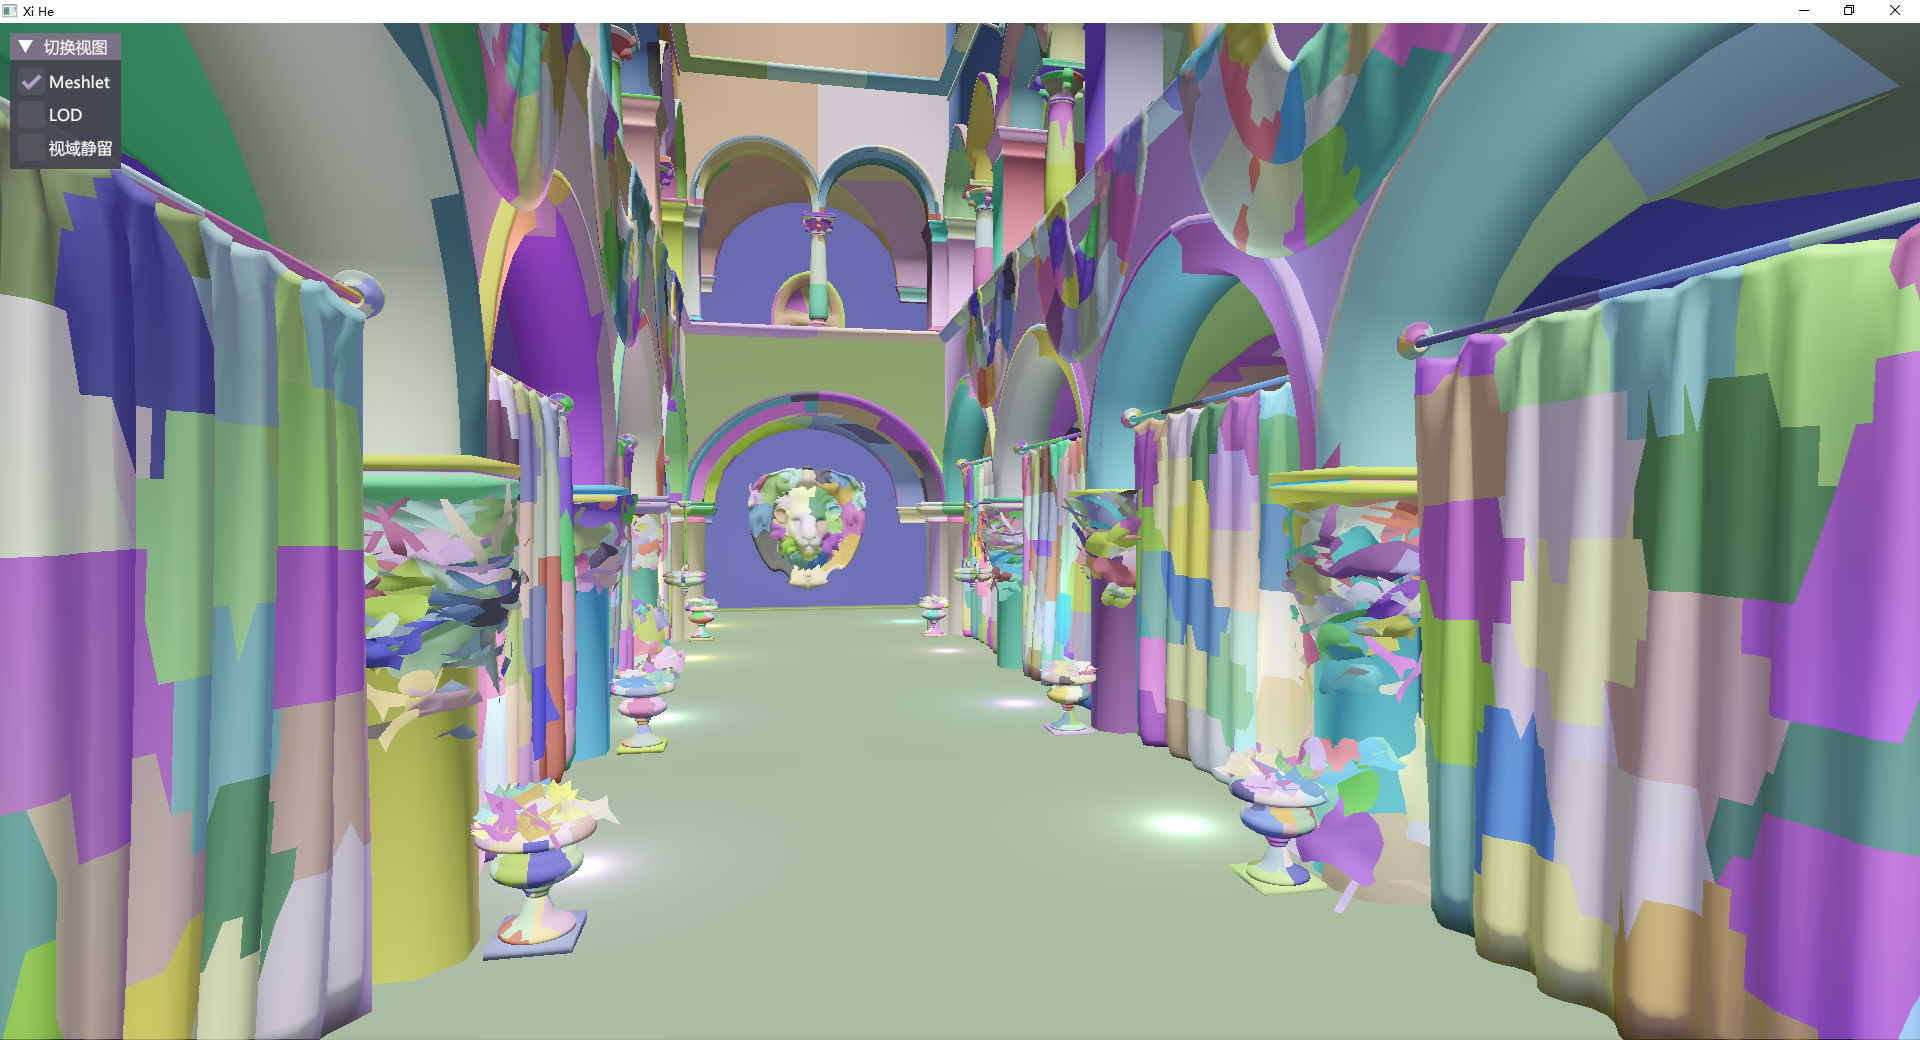
\includegraphics[width=\linewidth]{Meshlet.png}
    \caption{\label{fig:Meshlet}簇的可视化效果图}
\end{figure}

本项目对 Factory 场景设置了固定相机轨迹进行测试,
测量了不同剔除策略下的平均渲染帧时间,
以及 GPU 在裁剪阶段丢弃的平均图元数量。
GPU 在裁剪阶段丢弃的图元数量越多,
意味着处理了更多无效的几何数据,从而浪费了带宽和计算资源。
具体测试结果见\autoref{tab:culling}。

\begin{table}[ht]
    \caption{\label{tab:culling}不同剔除策略下的渲染性能测试结果}
    \begin{tabularx}{\linewidth}{|c|X<{\centering}|c|}
        \hline
        剔除策略 & GPU 在裁剪阶段丢弃的图元数 & 渲染帧时间 \\ \hline
        不使用剔除 & 40713.9k & 240.7ms \\ \hline
        使用实例级剔除 & 40350.5k & 233.5ms \\ \hline
        使用视锥剔除 & 28557.5k & 147.9ms \\ \hline
        使用圆锥剔除 & 39249.1k & 230.7ms \\ \hline
        同时使用视锥剔除和圆锥剔除 & 27575.3k & 142.7ms \\ \hline
    \end{tabularx}
\end{table}

从上述数据可以看出,实例级的剔除对于工业大场景的性能提升有限,
而基于簇的视锥剔除和圆锥剔除能够有效减少绘制三角形的数量。
二者相结合的基于簇的剔除策略显著提升了渲染帧率,
证明了基于簇的渲染方法在提高渲染效率方面的有效性。

\section{LOD机制}

\subsection{引言}

LOD(Level of Detail,细节层次)是一种通过根据物体与视点的距离
调整其细节程度的技术。
当物体距离视点较远时,可以使用较低的细节模型,
而当物体接近视点时,则使用更高细节的模型。
这种技术能显著减少不必要的计算量,提高渲染性能。
而在本项目中,LOD不仅用于提高渲染性能,
还与流式加载结合,进一步降低了显存占用。
通过按需加载不同细节层次的模型,本项目能够在保证画面质量的同时,
优化显存资源的使用。

\subsection{LOD生成} \label{subsec:LOD generation}

LOD 生成部分参考了 Nanite 的核心思想,整体过程大致可以分为以下几步:

\newcommand{\stepref}[1]{\textbf{Step~\ref{#1}}}

\begin{enumerate}
    \item 将初始模型划分为簇;
    \item 根据簇之间的连接性,将簇组织成簇组,每个簇组最多包含 16 个簇;
    \item 对每个簇组进行独立简化,确保每个簇组的边界完整,
    从而避免不同 LOD 之间出现裂缝;
    \item 将简化后的簇组重新划分为新的簇;
    \item 如果新的簇数量仍然过多,则返回步骤 2 进行进一步简化;
    否则,结束生成过程。
\end{enumerate}

其中,步骤 1 已经在 \ref{subsubsec:cluster division} 节中,
通过使用 MeshOptimizer 库得到了有效解决。
步骤 4 也可以采用类似的方法来处理。

对于步骤 2,本项目将生成的簇进一步划分为簇组。
理想情况下,我们希望簇组与簇组之间的共享边尽可能少,
这样可以最大限度地减少步骤 3 中锁定的顶点数量。
这一区域划分问题可以通过使用 METIS 库来有效解决。

划分完成后,对于每个簇组,将继续使用 MeshOptimizer 库进行简化,
即步骤 3。简化结束后,MeshOptimizer 库会返回一个误差值,
用以表示简化后的网格与原网格的相对误差。
该误差值将在 \ref{subsec:run-time lod select} 节中用于运行时的 LOD 选择。

为了确保简化过程能够顺利进行,还需要将距离较近的顶点进行合并。
这是因为,在处理拓扑不一致或具有多个接缝的网格时,
简化器可能会“卡住”,无法顺利完成简化任务。
顶点合并能够有效推动简化器去除更多的三角形,
从而促进简化过程。

为了高效地查找每个顶点的最近邻,
本项目采用了 K-D 树进行管理。
K-D 树的构建时间复杂度为 $O(N\log N)$,
查询时间复杂度为 $O(\log N)$,具有较高的效率。

此外,为了避免顶点合并后簇组的视觉误差过大,
本项目不仅考虑顶点之间在空间中的距离,
还将纹理坐标、法向量等其他因素纳入考虑范围。

在以上所有步骤完成后,不同 LOD 等级的簇将组成一个有向无环图(DAG),
如 \autoref{fig:DAG} 所示。
接下来的运行时阶段,本项目将利用该有向无环图进行 LOD 选择。

\begin{figure}[ht]
    \centering
    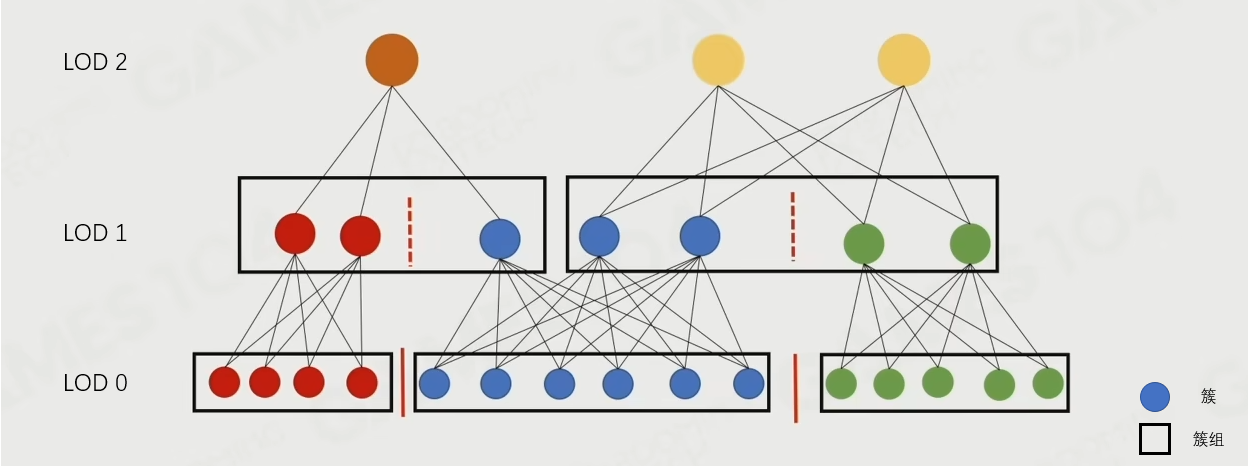
\includegraphics[width=\linewidth]{DAG.png}
    \caption{\label{fig:DAG}LOD的DAG示意图}
\end{figure}

\subsection{运行时 LOD 选择} \label{subsec:run-time lod select}

\par 对于 \autoref{fig:DAG} 中的有向无环图,
若在运行时遍历以进行 LOD 选择,开销将会较大。  
这是因为传统的遍历方式缺乏并发性,无法直接在 GPU 上执行。  
为了实现 LOD 选择的并行化,本项目对每个节点(簇)独立进行 LOD 选择。  
为此,需要在 LOD 生成阶段预先维护每个节点(簇)的误差值、包围球,
以及其父节点的误差值和包围球信息。

在运行时,基于这些预计算的数据,
本项目计算每个节点自身在屏幕空间上的误差 $cluster\_error$,  
以及其父节点在屏幕上的误差 $parent\_error$。
与此同时,本项目设置了一个阈值 $lod\_threshold$,  
当且仅当 $cluster\_error < lod\_threshold$ 
且 $parent\_error \geq lod\_threshold$ 时,该节点(簇)才有可能被绘制。

这种基于簇的 LOD 选择方法不仅保证了并行化,
还可以与基于簇的剔除(参见 \ref{subsubsec:cluster culling})  
在任务着色器中一同完成,避免了新增额外渲染通道的需求。  
这一方式有效降低了代码复杂度,并大幅提升了渲染效率。

\subsection{测试分析报告}

本项目首先使用 Sponza 场景的一部分,
对 LOD 生成的效果进行了测试,如\autoref{fig:LOD generation} 所示。
各级 LOD 对应的顶点数、三角形数和簇数如\autoref{tab:LOD} 所示。

\begin{figure}[!htb]
    \centering
    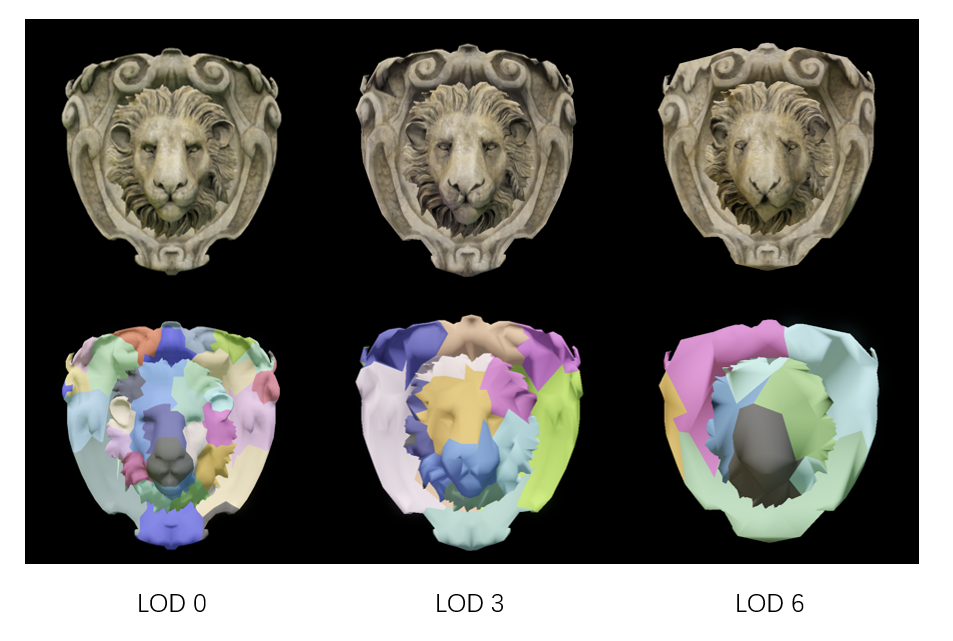
\includegraphics[width=\linewidth]{LOD生成.png}
    \caption{\label{fig:LOD generation}各级 LOD 的生成效果图}
\end{figure}

\begin{table}[!htb]
    \caption{\label{tab:LOD}各级 LOD 对应的顶点数、三角形数和簇数}
    \begin{tabularx}{\linewidth}{|X<{\centering}|X<{\centering}|X<{\centering}|X<{\centering}|}
        \hline
        LOD级别 & 顶点数 & 三角数 & 簇数 \\ \hline
        LOD 0 & 5032 & 7128 & 80 \\ \hline
        LOD 3 & 2223 & 2997 & 36 \\ \hline
        LOD 6 & 1108 & 1264 & 18 \\ \hline
    \end{tabularx}
\end{table}

从上述数据可以看出,LOD 生成的核心功能基本实现,
随着 LOD 级别的增大,顶点数、三角形数和簇数
都有了明显下降,效果良好。

此外,本项目还对运行时 LOD 的选择进行了简单测试,效果如


\section{流式加载}

\subsection{引言}

流式加载是一种按需加载的技术,
其核心思想是根据当前视野或者需求动态加载资源,
以减少内存占用和提高性能。
相比于传统的预加载方式,流式加载能有效避免一次性加载过多数据,
减少了显存压力,提升了渲染性能。

在本项目中,流式加载体现在两个方面:
一是对于不在屏幕中的物体,可以暂不加载,
从而避免了加载无效数据带来的显存开销;
二是对于远处的物体,可以只加载其粗糙的LOD模型,
进一步减少显存的使用。

因此,本项目在预处理阶段将场景数据转化为易于流式加载的形式,
并将其分页存储在CPU内存中;
在运行时阶段,系统会根据需求动态加载所需的场景数据页到GPU上,
确保在维持渲染效果的同时,
有效优化显存的使用效率。

\subsection{场景数据的存储}

为了提高运行时动态加载效率,  
本项目在预处理阶段存储场景数据,并按页划分。  
数据存储以簇组为单位,  
因为任务着色器中的剔除和 LOD 选择是以簇组为单位进行的。  
即,一个簇组要么完全渲染,要么完全不渲染。
当一个簇组需要渲染时,  
只需加载该簇组所在的页到 GPU 中。  
按簇组存储顶点和索引信息,  
有助于提高空间局部性(spatial locality),  
减少数据交换频率,有效降低页表压力,并提升 GPU 显存利用率。

\subsection{动态加载}

在任务着色器中,所有簇组都需要经过剔除和 LOD 选择操作,只有通过这两个测试的簇组才会被渲染并加载到 GPU 显存中。因此,在 GPU 的任务着色器中,需要记录每个待渲染簇组对应的数据页编号,并将这些编号传回给 CPU。CPU 使用一个页表来管理这些数据页,并通过 Vulkan 的稀疏资源特性实现数据页的动态绑定。

\subsubsection{页表的管理}

在本项目中,页表的容量和数据页的大小都是固定的。每个页表条目对应一个显存块。当 GPU 请求新的数据页时,CPU 会检查页表是否有空闲位置。如果没有空闲位置,则会选择一个当前未使用的数据页进行换出。页表的示意图如 \autoref{fig:page table} 所示。

\begin{figure}[!htb]
    \centering
    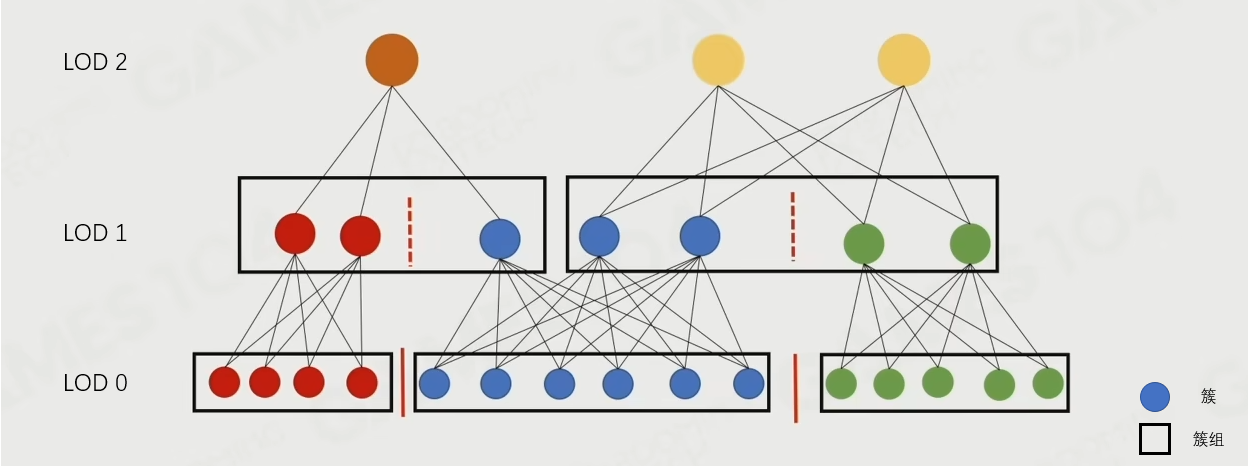
\includegraphics[width=\linewidth]{DAG.png}
    \caption{\label{fig:page}页表示意图}
\end{figure}

目前,本项目实现了两种数据页换入换出策略:一种是随机替换策略,当页表已满时,随机选择一个未在当前帧使用的数据页进行换出;另一种是 LRU(最近最少使用)替换策略,它选择最近最少使用的数据页进行换出。在 \ref{subsec:streaming test} 中,我们将对这两种策略的性能进行比较。

在极端情况下,若当前视角需要加载的场景数据过多,而页表中的所有数据页都已被当前帧使用,导致无法换入新的数据页,可能会造成场景中的空洞。为应对这种情况,本项目借鉴了类似于拥塞控制的思路(此处可引用),当页表压力过大时,会适当降低 LOD 选择的标准,即提高 \ref{subsec:run-time lod select} 中提到的 $lod_threshold$,采取更为激进的 LOD 选择策略。即使是距离相机较近的物体,也可能会选择较为粗糙的 LOD。而当页表压力恢复到正常水平时,可以逐步恢复原有的 LOD 选择策略。虽然这种策略会略微降低画面质量,但能有效避免场景中出现空洞,保持页表的稳定运行。

\subsubsection{稀疏资源}

稀疏资源是 Vulkan 1.2 引入的一个重要特性,主要用于虚拟几何、虚拟纹理等场景。传统的 Vulkan 资源需要连续、完整地绑定到单个显存块,并且在生命周期内绑定关系无法修改。而稀疏资源打破了这些限制,它不仅支持将资源分布到多个显存块,还允许在运行时动态修改绑定关系。这一特性为实现高效的动态加载提供了极大的便利。

在本项目中,我们利用 Vulkan 的稀疏资源功能,创建了一个非常大的缓冲区来存储场景数据。该缓冲区按页划分并绑定到不同的显存块上。部分缓冲区位置甚至没有存储任何数据,以节省显存空间。如 \autoref{fig:page table} 所示,页表管理着每个数据页的加载状态。

需要注意的是,Vulkan 对缓冲区的最大大小有限制。因此,这个逻辑上的缓冲区实际上由多个大小相同的缓冲区组成。在网格着色器中,只需根据当前需要的数据页,计算其所在的缓冲区位置即可。而在任务着色器阶段,我们确保网格着色器只会访问已加载数据的部分,避免访问到未加载的空白区域。

\subsection{测试分析报告} \label{subsec:streaming test}

可以测试LRU、随机两种不同方法的time、换入换出次数等
还可以测试Page Size大小的影响

\section{项目成果}

\section{Overleaf 使用注意事项}

如果你在Overleaf上编译本模板,请注意如下事项~\cite{zjuthesis}: